\begin{exercise}
      {ID-bd6ae08172fe6cbe9973365cbc8f8d50c6b8e92b}
      {Rubbellose}
  \ifproblem\problem\par
    % <PROBLEM>
    \hangindent4cm%
    \hangafter-7%
    \raisebox{1.66ex}[0pt][0pt]%
    {%
      \raisebox{-3cm}[0pt][0pt]%
      {%
        \makebox[0pt][r]%
        {%
          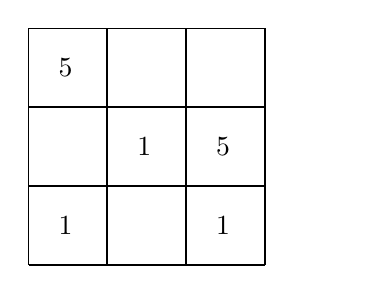
\begin{tikzpicture}[line width=0.6pt]
            \draw (0, 0) grid (3, 3);
            \clip (0, 0) rectangle (4, 3);
            \begin{scope}[xshift=-0.5cm, yshift=-0.5cm]
              \node at (1, 3) {5\,\officialeuro};
              \node at (2, 2) {1\,\officialeuro};
              \node at (3, 2) {5\,\officialeuro};
              \node at (1, 1) {1\,\officialeuro};
              \node at (3, 1) {1\,\officialeuro};
            \end{scope}
          \end{tikzpicture}%
        }%
      }%
    }%
    An einem Lotteriestand werden Rubbellose
    angeboten. Von den neun Feldern eines Loses
    tragen drei den Auszahlungsbetrag 1 Euro
    und zwei den  Auszahlungsbetrag 5 Euro.
    Die restlichen vier Felder sind Leerfelder.
    Die Lage der einzelnen Felder ist zufällig.
    Die Skizze zeigt ein mögliches Beispiel.
    Jedes Feld ist mit einer undurchsichtigen
    Deckschicht überzogen, die man mit einer
    Münze entfernen kann.
    \par
    Ein Spiel ist wie folgt definiert:
    Nach dem Kauf eines Rubbelloses muss der
    Käufer genau zwei Felder freirubbeln,
    d.\,h. die Deckschicht dieser beiden
    Felder entfernen, so dass der Inhalt
    der Felder sichtbar wird.
    \begin{enumerate}[a)]
      %\setlength{\itemsep}{-1ex}%
      \item Zeichnen Sie ein geeignetes Baumdiagramm
            für ein Spiel mit den zugehörigen
            Wahrscheinlichkeiten folgender Ereignisse:
            \begin{enumerate}[A:]
              \setlength{\itemsep}{-1ex}%
              \item Beide Felder sind leer.
              \item Beide Felder zeigen einen
                    Geldbetrag an.
              \item Höchstens ein Feld zeigt einen
                    Geldbetrag an.
              \item Beide Felder zusammen zeigen
                    einen Geldbetrag von mindestens
                    6 Euro an.
            \end{enumerate}
      \item Ein Rubbellos kostet 3 Euro. Es
            werden die Geldbeträge der
            freigerubbelten Felder ausgezahlt.
            Für Leerfelder gibt es nichts.
            Erstellen Sie eine Tabelle für
            alle möglichen Auszahlungsbeträge.
            \par
            Welchen Gewinn kann der Betreiber
            des Lotteriestandes im Durchschnitt
            bei 10 Spielen erwarten?
            Wie viele Rubbellose müssen täglich
            verkauft werden, damit der Betreiber
            in 7 Tagen mindestens 300 Euro Gewinn
            erzielt?
      \item Wie muss der Auszahlungsbetrag für
            die zwei 5-Euro-Feldern abgeändert
            werden, damit bei einem unveränderten
            Preis von 3 Euro pro Rubbellos und
            allen anderen unveränderten Gewinnen
            das Spiel fair wird?
      \item Berechnen Sie die Wahrscheinlichkeit dafür,
            dass bei 20 Spielen, in denen nur ein Feld
            freigerubbelt wird
            \begin{enumerate}[A:]
              \setlength{\itemsep}{-1ex}%
              \item genau 5 mal 1 Euro erreicht wird.
              \item mindestens 3 mal 1 Euro erreicht wird.
              \item höchstens 7 mal 1 Euro erreicht wird.
              \item mindestens 2 mal und höchstens 5 mal 1 Euro erreicht wird.
            \end{enumerate}
    \end{enumerate}
    % </PROBLEM>
  \fi
  %\ifoutline\outline\par
    % <OUTLINE>
    % </OUTLINE>
  %\fi
  %\ifoutcome\outcome\par
    % <OUTCOME>
    % </OUTCOME>
  %\fi
\end{exercise}
